\documentclass[12pt, letterpaper]{article}
\usepackage{listings}
\usepackage{graphicx}
\usepackage{color}
\usepackage{caption}
\usepackage{subcaption}
\usepackage{hyperref}
\usepackage{fancyhdr}
\usepackage{mathrsfs}
\usepackage[margin=3cm]{geometry}
\usepackage[dvips]{epsfig}
\usepackage{placeins}
\usepackage{longtable}
\usepackage{wrapfig}
\usepackage{caption}
\usepackage{alltt}

\setlength{\parindent}{0.0in}
\setlength{\parskip}{0.05in}

\definecolor{dkgreen}{rgb}{0,0.6,0}
\definecolor{gray}{rgb}{0.5,0.5,0.5}
\definecolor{mauve}{rgb}{0.58,0,0.82}
\definecolor{deepblue}{rgb}{0,0,0.7}
\definecolor{deepred}{rgb}{0.6,0,0}
\definecolor{deepgreen}{rgb}{0,0.5,0}
\definecolor{red}{rgb}{0.9,0,0}

\newcommand\course{CS532}
\newcommand\semester{Spring 2017}
\newcommand\hwnum{10}
\newcommand\yourname{Justin Schaffner}
\newcommand\login{JASchaff}
\newenvironment{answer}[1]{\subsection*{Problem #1}}

\pagestyle{fancyplain}
\headheight 40pt
\lhead{\yourname\ (\login)\\\course\ --- \semester}
\chead{\textbf{\Large Assignment \hwnum}}
\rhead{\today}
\headsep 40pt

\DeclareCaptionFont{white}{\color{white}}
\DeclareCaptionFormat{listing}{\colorbox[cmyk]{0.43, 0.35, 0.35,0.01}{\parbox{\dimexpr\textwidth-2\fboxsep\relax}{#1#2#3}}}
\captionsetup[lstlisting]{format=listing,labelfont=white,textfont=white, singlelinecheck=false, margin=0pt, font={bf,footnotesize}}
\captionsetup[figure]{format=listing,labelfont=white,textfont=white, singlelinecheck=false, margin=0pt, font={bf,footnotesize}}
\captionsetup[alltt]{format=listing,labelfont=white,textfont=white, singlelinecheck=false, margin=0pt, font={bf,footnotesize}}



\lstnewenvironment{MyBash}[1][]{\noindent\lstset{#1, language=bash, aboveskip=3mm, belowskip=3mm, showstringspaces=false, columns=flexible, basicstyle={\small\ttfamily}, numbers=none, numberstyle=\tiny\color{grey}, keywordstyle=\color{black}, commentstyle=\color{dkgreen}, stringstyle=\color{black}, breaklines=true, breakatwhitespace=true, tabsize=3, frame=tb }}{}
\lstnewenvironment{MyPython}[1][]{\noindent\lstset{#1, language=Python, aboveskip=3mm, belowskip=3mm, basicstyle=\small, otherkeywords={self}, keywordstyle=\color{deepblue}, emph={MyClass,__init__}, emphstyle=\color{deepred}, stringstyle=\color{deepgreen}, commentstyle=\color{red}, frame=tb, showstringspaces=false, breaklines=true }}{}
\lstnewenvironment{MyR}[1][]{\noindent\lstset{#1, language=R, aboveskip=3mm, belowskip=3mm, basicstyle=\small, breaklines=true, frame=tb}}{}

\begin{document}

\begin{answer}{1: KNNEstimate of Blog-Term Matrix}
Q1: Using the data from A8:
- Consider each row in the blog-term matrix as a 1000 dimension vector,
corresponding to a blog.
- From chapter 8, replace numpredict.euclidean() with cosine as the
distance metric. In other words, you'll be computing the cosine between
vectors of 1000 dimensions.
- Use knnestimate() to compute the nearest neighbors for both: \url{http://f-measure.blogspot.com/}   \url{http://ws-dl.blogspot.com/}  for k={1,2,5,10,20}.\\
Answer: Getting the rows from the A8 blogterm matrix as vectors was fairly simple. I pulled the blognames and vectors from the file, zipped them into a list of tuples, then turned them into a dictionary of blognames: vectors. Then I extracted F-measure and WS-DL from that dictionary and put them in their own list for comparison. That can be seen in Listing \ref{lst:tenmain} in the first section. The KNNEstimate() function had to be adjusted, since we're not trying to find average wine prices. For cosine, I used scipy.py spatial.distance.cosine(). The 3 functions involved are cosine() getdistances() and knnestimate() from ten\textunderscore dimension.py in Listing \ref{lst:tendimension}. The only adjustment I had to make, other than cosine, was in distancelist.sort() in getdistances(). I added reverse=True, so that the closest would be at the top of the list, rather than at the bottom. The results for Question 1 can be seen in Listing \ref{lst:q1results} and in Problem1Output.txt . The nearest neighbors calculated for F-measure were not only similar to those nearest in the dendrogram from A8, but just looking at them one can tell that they are for the most part topically similar. Those placed near WS-DL are also similar to the A8 dendrogram, though one can't be sure about the topicality of them just from their titles.

\begin{MyBash}[caption=Q1 Results, label=lst:q1results]
Nearest Neighbors to F-Measure for k=1
	SPIN IT RECORDS Moncton 467A Main Street Moncton NB CANADA
Avg Distance 0.680835
Nearest Neighbors to F-Measure for k=2
	SPIN IT RECORDS Moncton 467A Main Street Moncton NB CANADA
	Indie Top 20 - The Blog!
Avg Distance 0.539775
Nearest Neighbors to F-Measure for k=5
	SPIN IT RECORDS Moncton 467A Main Street Moncton NB CANADA
	Indie Top 20 - The Blog!
	.
	MTJR RANTS & RAVES ON MUSIC
	The Power of Independent Trucking
Avg Distance 0.418254
Nearest Neighbors to F-Measure for k=10
	SPIN IT RECORDS Moncton 467A Main Street Moncton NB CANADA
	Indie Top 20 - The Blog!
	.
	MTJR RANTS & RAVES ON MUSIC
	The Power of Independent Trucking
	Swinging Singles Club
	Subterranean Noise
	KiDCHAIR
	DaveCromwell Writes
	Eli Jace | The Mind Is A Terrible Thing To Paste
Avg Distance 0.344340
Nearest Neighbors to F-Measure for k=20
	SPIN IT RECORDS Moncton 467A Main Street Moncton NB CANADA
	Indie Top 20 - The Blog!
	.
	MTJR RANTS & RAVES ON MUSIC
	The Power of Independent Trucking
	Swinging Singles Club
	Subterranean Noise
	KiDCHAIR
	DaveCromwell Writes
	Eli Jace | The Mind Is A Terrible Thing To Paste
	Coyote Doc Music Co-op
	Encore
	Some Call It Noise....
	www.doginasweater.com Live Show Review Archive
	The Jeopardy of Contentment
	Stereo Pills
	GYPSY RHAPSODY
	Cuz Music Rocks
	The Girl at the Rock Show
	The Music Binge
Avg Distance 0.288265
Nearest Neighbors to Web Science and Digital Libraries Research Group for k=1
	The Grunge Pit
Avg Distance 0.723314
Nearest Neighbors to Web Science and Digital Libraries Research Group for k=2
	The Grunge Pit
	hmmhannah
Avg Distance 0.633799
Nearest Neighbors to Web Science and Digital Libraries Research Group for k=5
	The Grunge Pit
	hmmhannah
	macthemost
	Riley Haas' blog
	ORGANMYTH
Avg Distance 0.491994
Nearest Neighbors to Web Science and Digital Libraries Research Group for k=10
	The Grunge Pit
	hmmhannah
	macthemost
	Riley Haas' blog
	ORGANMYTH
	The Ideal Copy
	Subterranean Noise
	PALMIRA A PISTA TRES
	Diagnosis: No Radio
	Eli Jace | The Mind Is A Terrible Thing To Paste
Avg Distance 0.377691
Nearest Neighbors to Web Science and Digital Libraries Research Group for k=20
	The Grunge Pit
	hmmhannah
	macthemost
	Riley Haas' blog
	ORGANMYTH
	The Ideal Copy
	Subterranean Noise
	PALMIRA A PISTA TRES
	Diagnosis: No Radio
	Eli Jace | The Mind Is A Terrible Thing To Paste
	.
	DaveCromwell Writes
	Some Call It Noise....
	Avidd Wallows' Blog
	The Power of Independent Trucking
	Hip In Detroit
	simone goes
	Stories From the City, Stories From the Sea
	Mile In Mine
	MTJR RANTS & RAVES ON MUSIC
Avg Distance 0.296337

\end{MyBash}

\end{answer}

\begin{answer}{2: LIBSVM for Blog Entry Classification}
Q2: Rerun A9, Q2 but this time using LIBSVM. If you have n categories, you'll have to run it n times. For example, if you're classifying music and have the categories: metal, electronic, ambient, folk, hip-hop, pop you'll have to classify things as: metal / not-metal electronic / not-electronic ambient / not-ambient etc.\\
Use the 1000 term vectors describing each blog as the features, and your manually assigned classifications as the true values. Use 10-fold cross-validation (as per slide 46, which shows 4-fold cross-validation) and report the percentage correct for each of your categories.\\
Answer: This one was more difficult, mainly in that the LIBSVM library wouldn't install properly. I ended up placing the library in the working folder, running make within the necessary folders using the given makefile, then placing an empty \textunderscore \textunderscore init\textunderscore \textunderscore .py in those folders so Python would recognize it as a Python directory. I also had to change the import calls for svm within svmutil.py . I got the idea for the solution from a stack exchange post, and it worked out pretty well. As far as following the code from the book, the LIBSVM library has changed a bit. The cross-validation function is now built into the svm\textunderscore train() function, and passing the option is less straightforward than just saying ``cross validation = True". The documentation could be more helpful. Eventually I just opened up svm.py and found what the parameter function was expecting, though the list of options was actually in svmutil.py . Go figure. Once that was sorted, the rest was fairly easy. I adjusted the myread() function from A9 to return a dictionary of title: term-count vectors. This can be found in Listing \ref{lst:tendimension}. tenMain then creates an answer list of (1,-1) for each category, feeding them both into svm\textunderscore train(). svm\textunderscore train() returns the percentage correct, so no further calculation needs to be done. The results can be found in Table \ref{q2results} and the raw data in Question2Output.txt . LIBSVM yields a much better result than the Fisher Method from A9. Using the same data and categories, the accuracy of prediction was much higher. 

\begin{table}[!htbp]
\small
\centering
\caption{Q2 Results}
\label{q2results}
\resizebox{\textwidth}{!}{
\begin{tabular}{ll}
Category	&  Percent Correct\\
how-to	&  84\\
opinion	& 97\\
community	&  79\\
recommendations-travel	&  90\\
recommendations-gear	&  67\\
recommendations-media	&  92\\
news	&  91
\end{tabular}
}
\end{table}

\end{answer}

\begin{answer}{3: 1000 TimeMaps Comparison}
Q3: Re-download the 1000 TimeMaps from A2, Q2. Create a graph where the x-axis represents the 1000 TimeMaps. If a TimeMap has "shrunk", it will have a negative value below the x-axis corresponding to the size difference between the two TimeMaps. If it has stayed the same, it will have a "0" value. If it has grown, the value will be positive and correspond to the increase in size between the two TimeMaps. As always, upload all the TimeMap data. If the A2 github has the original TimeMaps, then you can just point to where they are in the report.\\
Answer: I was able to reuse my functions from A2 with a small adjustment to return only the TimeMap rather than both the TimeMap and the CarbonDate age. These can be found in Listing \ref{lst:tendimension} in the third section. tenMain.py in Listing \ref{lst:tenmain} pulls the old data from the file old\textunderscore data\textunderscore set.txt and zips it into a dictionary with the url links from twitter\textunderscore links.txt . It then loops through the links and gets the updated memento count, storing the old count, new count, and their difference in data\textunderscore set.txt . Only a few of the Time Maps had shrunk, while many had grown larger, and a lot had stayed the same. Two of the links had a difference in the thousands. The results are in Figure \ref{q3results} and the rcode in Listing \ref{lst:q3rcode}.

\begin{figure}
\caption{Q3 TimeMaps}
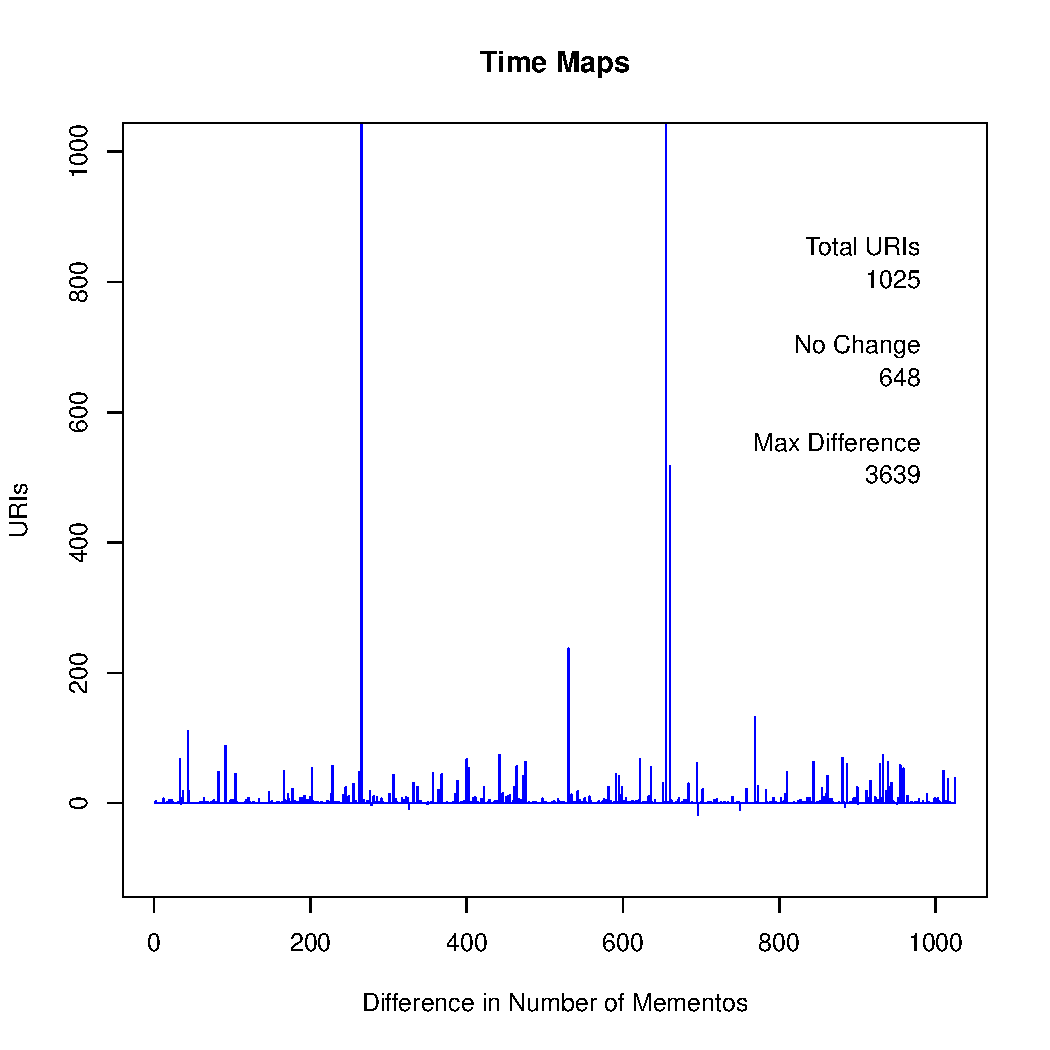
\includegraphics[width=\textwidth, height=0.95\textheight, keepaspectratio]{diff_data}
\label{q3results}
\end{figure}

\begin{MyR}[caption=Q3 R code, label=lst:q3rcode]
require(graphics)

pdf("Desktop/mem_data.pdf")

data_table<-read.table(file="Desktop/Assign_10_CS_532/data_set.txt", header=T, sep="\t")

diff_data<-c(data_table$diff)

max_diff<-max(diff_data)

num_zero_diff<- length(diff_data[diff_data==0])

plot(diff_data, xlim= c(1, 1025), ylim=c(-100,1000), pch=20, col='blue', main="Time Maps", xlab="Difference in Number of Mementos", ylab="URIs", type='h')

text(c(1000,1000,1000,1000,1000,1000),c(850,800,700,650,550,500), labels=c("Total URIs", length(diff_data), "No Change", num_zero_diff, "Max Difference", max_diff), pos=2, col='black')

dev.off()
\end{MyR}

\end{answer}

\FloatBarrier
\begin{MyPython}[caption=tenMain.py, label=lst:tenmain]
from ten_dimension import *
from libsvm.python import svm
from libsvm.python import svmutil as svmu
import feedparser
import os



#Question 1
(rownames, colnames, vectors)=readfile('blogdata.txt')

data=dict(zip(rownames, vectors))

Vec={}
klist=[1,2,5,10,20]
for key, value in data.items():
    if key == 'F-Measure':
        Vec.setdefault(key, value)
    if key == 'Web Science and Digital Libraries Research Group':
        Vec.setdefault(key, value)
for key in Vec.keys():
    del data[key]


for key, value in Vec.items():
    for k in klist:
        print('Nearest Neighbors to %s for k=%d' % (key, k))
        print('Avg Distance %f' % knnestimate(data, value, k))
        
del data, Vec, klist, rownames, colnames, vectors

#|||||||||||||||||||||||||||||||||||||||||||||||
#Question 2
articles={}
categories=[]
for line in open('groundtruth.txt', 'r'):
    (title, actual)=line.split('\t')
    articles.setdefault(title,actual.rstrip())
    if actual.rstrip() not in categories:
        categories.append(actual.rstrip())

data=myread(articles, './feeds')
for cat in categories:
    vectors=[]
    answers=[]
    for title, answer in articles.items():
        if answer==cat:
            answers.append(1)
        else:
            answers.append(-1)
        vectors.append(data[title])
    prob=svm.svm_problem(answers, vectors)
    param=svm.svm_parameter('-t 2 -v 10')
    
    correct=svmu.svm_train(prob, param)
    print('Category: %s \n\t Percent Correct: %d' %(cat, correct))    
    
#||||||||||||||||||||||||||||||||||||||||||||||
#Question 3

old_data=[]
with open("old_data_set.txt", 'r') as olddata:
    for line in olddata:
        old_data.append(line.split('\t')[0].rstrip())
links=[]
with open('twitter_links.txt', 'r') as linkfile:
    for line in linkfile:
        links.append(line.rstrip())

data=dict(zip(links, old_data))

with open('data_set.txt', 'w') as outfile:
    for key, value in data.items():
        new_count=get_data(key)
        print(value, new_count, (int(new_count)-int(value)), sep='\t', file=outfile)

\end{MyPython}

\begin{MyPython}[caption={ten\textunderscore dimension.py}, label=lst:tendimension]
import feedparser
import re
from math import sqrt
from scipy import spatial
import os
import requests
from urllib.parse import urljoin
from datetime import datetime
import json

#Q1 functions
def cosine(vec1, vec2):
    return float(1-spatial.distance.cosine(vec1,vec2))
    


def getdistances(data,vec1):
    distancelist=[]
    for key in data.keys():
        vec2=data[key]
        distancelist.append((cosine(vec1,vec2),key))
    distancelist.sort(reverse=True)
    return distancelist

def knnestimate(data,vec1,k=3):
    # Get sorted distances
    dlist=getdistances(data,vec1)
    avg=float(0.0)
    # Take the average of the top k results
    for i in range(k):
        idx=dlist[i][0]
        print('\t%s'% dlist[i][1])
        avg+=idx
    avg=avg/k
    return avg


def readfile(filename):
    lines=[line for line in open(filename, 'r')]
    # First line is the column titles
    colnames=lines[0].strip( ).split('\t')[1:]
    rownames=[]
    data=[]
    for line in lines[1:]:
        p=line.strip( ).split('\t')
        # First column in each row is the rowname
        rownames.append(p[0])
        # The data for this row is the remainder of the row
        data.append([float(x) for x in p[1:]])
    return rownames,colnames,data

#|||||||||||||||||||||||||||||||||||||||||
#Q2 functions


def myread(articles, path):
    entries=[]
    data={}
    words={}
    for file in os.listdir(path):
        feed=os.path.join(path, file)
        f=feedparser.parse(feed)
        for entry in f.entries:
            entries.append(entry)
    for entry in entries:
        if entry.title in articles.keys():
            wc=getwordcounts(entry)
            for key in wc.keys():
                words.setdefault(key,0)
                words[key]+=1
            data[entry.title]=wc
    #shortens word list to 1000 most used        
    wordtuple=[]
    for w,bc in words.items( ):
        #frac=float(bc)/len(articles)
        #if frac>0.1 and frac<.99:
        wordtuple.append((w, bc))
    wordtuple.sort(key=lambda x: x[1], reverse=True)
    wordlist=list(x[0] for x in wordtuple)
    if len(wordlist)>1000:
        del wordlist[1000:]
    del wordtuple
    del words
    #converts wordcounts to a vector
    for title, d in data.items():
        vector=[]
        for word in wordlist:
            if word in d:
                vector.append(d[word])
            else: vector.append(0)
        data[title]=vector
    print('Total Number of Words: %d' %len(wordlist))
            
    return data
    

# Returns title and dictionary of word counts for an RSS feed
def getwordcounts(entry):
    wc={}
    if 'summary' in entry:
        summary=entry.summary
    else:
        summary=entry.description
    # Extract a list of words
    words=getwords(entry.title+' '+summary)
    for word in words:
        wc.setdefault(word,0)
        wc[word]+=1
   
    return wc

def getwords(doc):
    splitter=re.compile('\\W*')
    # Split the words by non-alpha characters
    words=[s.lower( ) for s in splitter.split(doc) if len(s)>2 and len(s)<20]
    # Return the unique set of words only
    return words

#|||||||||||||||||||||||||||||||||||||||||
#Question 3 functions

def get_aggregate(uri):
    aggregate='http://memgator.cs.odu.edu/timemap/link/'.rstrip()
    uri=aggregate+uri.rstrip()
    tbody=requests.get(uri)
    print(tbody.status_code)
    if not(tbody.status_code == 200):
        raise StopIteration
    for line in tbody:
        yield line
                
def get_data(uri):
    num_mementos=0
    for line in get_aggregate(uri):
        if b'memento' in line:
            num_mementos+=1
    return num_mementos
\end{MyPython}


\end{document}



\begin{answer}{1: Build the Data Set}

\end{answer}


\begin{MyPython}[caption=Q1 getRSS.py, label=lst:getrss]

\end{MyPython}

\begin{table}[!htbp]
\small
\centering
\caption{50/50 Results}
\label{5050}
\resizebox{\textwidth}{!}{
\begin{tabular}{lll}

\end{tabular}
}
\end{table}

\FloatBarrier
\begin{longtable}{llll}
\small
\caption{10-fold FPR}\\
\label{1010FRP}\\

\end{longtable}
\FloatBarrier

\begin{figure}
\caption{Q2 Dendrogram}
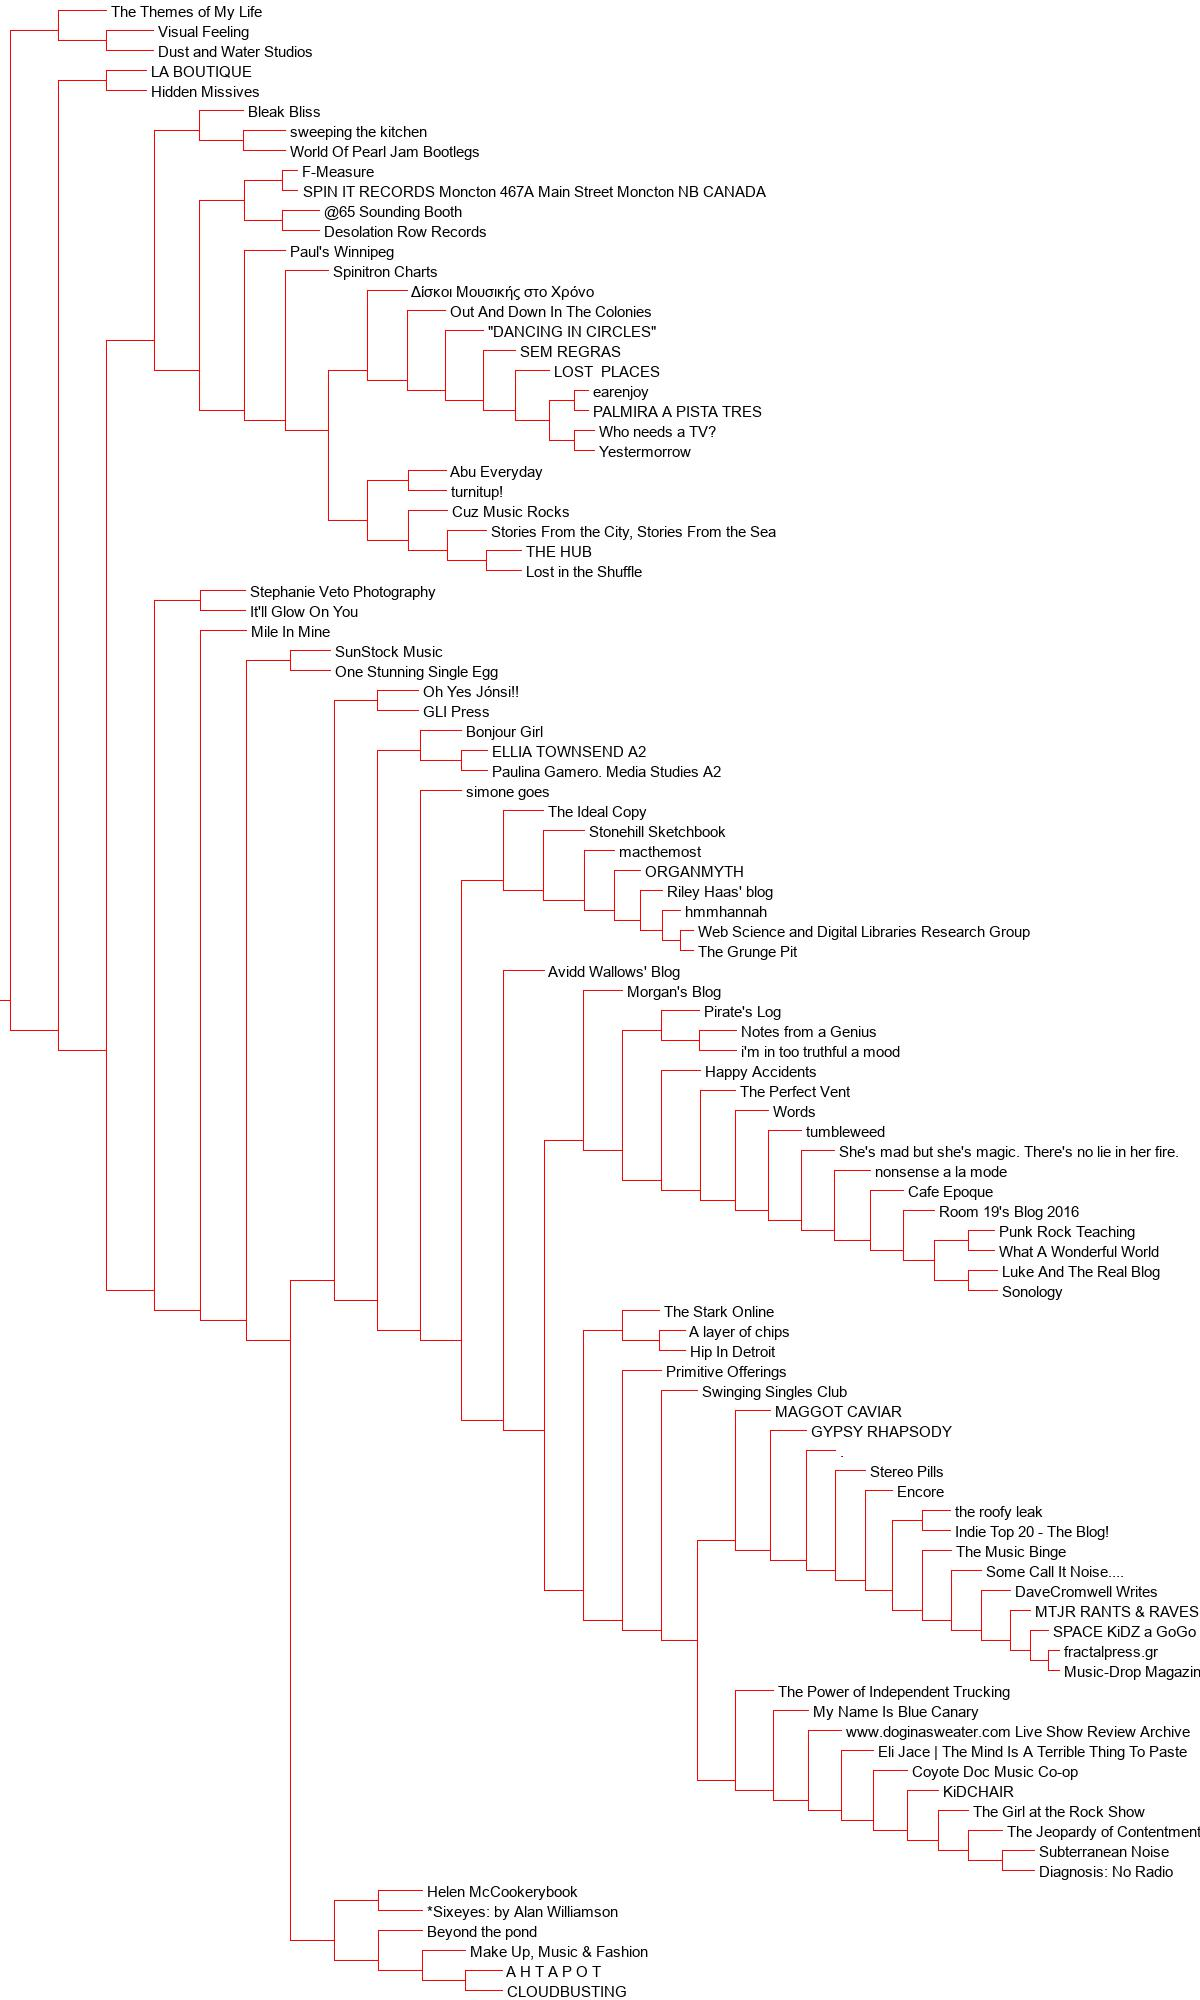
\includegraphics[width=\textwidth, height=0.95\textheight, keepaspectratio]{1blogclust}
\label{dendrogram1}
\end{figure}






